\documentclass[aps, superscriptaddress]{revtex4} 

\usepackage[switch]{lineno}
\usepackage{amsmath}
\usepackage{amssymb}
\usepackage{empheq}
\usepackage[parfill]{parskip}
\usepackage[active]{srcltx}
\usepackage{color}
\usepackage{array}
\usepackage{subcaption}
\usepackage{booktabs}
\usepackage{amsfonts}
\usepackage{dsfont}
\usepackage{graphicx}
\usepackage{csquotes}
\usepackage{float}
\usepackage{ragged2e}
\usepackage[pdftex, pdftitle={Article}, pdfauthor={Author}]{hyperref} % For hyperlinks in the PDF

\hypersetup{
    colorlinks=true,
    linkcolor=blue,
    citecolor=blue,
    urlcolor=blue
}

\begin{document}

\setlength{\parindent}{0.5cm}

\title{\textbf{Hyperuniformity in the Frustrated Vicsek-Kuramoto Model}}
\author{Yichen Lu}


\maketitle

\tableofcontents

% \newpage
\section{The Model}

Particles are described by position $\mathbf{r}_i=\left( x_i, y_i \right)$ and phase angle $\theta_i$, evolving as:
\begin{subequations} 
    \label{eq:totalDynamicsMeanField}
    \begin{align}
        \dot{\mathbf{r}}_i&=v\mathbf{p}\left( \theta _i \right)\;\label{eq:dotR},
        \\
        \dot{\theta}_i&=\frac{K}{\left| A_i \right|}\sum_{j\in A_i}{\left[ \sin \left( \theta _j-\theta _i+\alpha \right) -\sin \alpha \right]}\;\label{eq:dotTheta},
    \end{align}
\end{subequations}
where $A_i\left( t \right) =\left\{ j: \left| \mathbf{r}_i\left( t \right) -\mathbf{r}_j\left( t \right) \right|\leqslant d_0 \right\}$ is the set of neighbors within coupling radius $d_0$, $K \left(\geqslant 0\right)$ is coupling strength, and $\alpha$ is frustration.
The term $-\sin\alpha$ ensures synchronization ($\theta_j = \theta_i$) remains an equilibrium \cite{10.1143/PTP.79.1069}.
This model generalizes alignments \cite{PhysRevLett.119.058002,PhysRevResearch.1.023026,Escaff2020,PhysRevLett.127.238001,PhysRevLett.133.258302}, anti-alignments \cite{PhysRevE.109.024602,PhysRevE.110.024603}, and chimera states \cite{PhysRevE.98.032219,PhysRevE.102.022604}. It reduces to normal Vicsek–Kuramoto for $\alpha=0$ and anti-aligning interactions for $\alpha=\pi$.

A hyperuniform \cite{PhysRevE.68.041113,TORQUATO20181} (also known as superhomogeneous \cite{PhysRevD.65.083523}) point configuration is characterized by structure factor $S\left( \mathbf{q} \right)$ tends to zero as wavenumber $q\equiv \left| \mathbf{q} \right|\to 0$:
\begin{equation}
    \lim _{q\to 0}S\left( \mathbf{q} \right) =0,
    \label{eq:hyperuniformDefinition}
\end{equation}
indicating single scattering of incident radiation vanishes in the infinite-wavelength limit. 
Equivalently, the number variance $\sigma _N ^2\left( R \right)$ within a spherical observation window of radius $R$ grows more slowly than the window volume in large-$R$ limit:
\begin{equation}
    \lim _{R\to \infty}\frac{\sigma _N ^2\left( R \right)}{R^d}=0,
    \label{eq:hyperuniformDefinition_variance}
\end{equation}
where $d$ is the spatial dimension. 
The two definitions are linked via the relation \cite{PhysRevE.68.041113}:
\begin{equation}
    \sigma _N ^2\left( R \right) =\rho v_1\left( R \right) \left[ 1+\rho \int _{\mathbb{R} ^d}{h\left( \mathbf{r} \right) \alpha \left( r; R \right) d\mathbf{r}} \right],
    \label{eq:variance_structureFactor_relation}
\end{equation}
where $\rho$ is number density, $v_1\left( R \right)$ is the volume of a $d$-dimensional sphere of radius $R$, $h\left( \mathbf{r} \right)=g_2\left( \mathbf{r} \right) -1$ is the total correlation function with $g_2\left( \mathbf{r} \right)$ being the pair correlation function, and $\alpha \left( r; R \right)$ is the scaled intersection volume of two spheres of radius $R$ separated by distance $r$.

\newpage
\section{Simulation Results}

\begin{figure}[H]
    \centering
    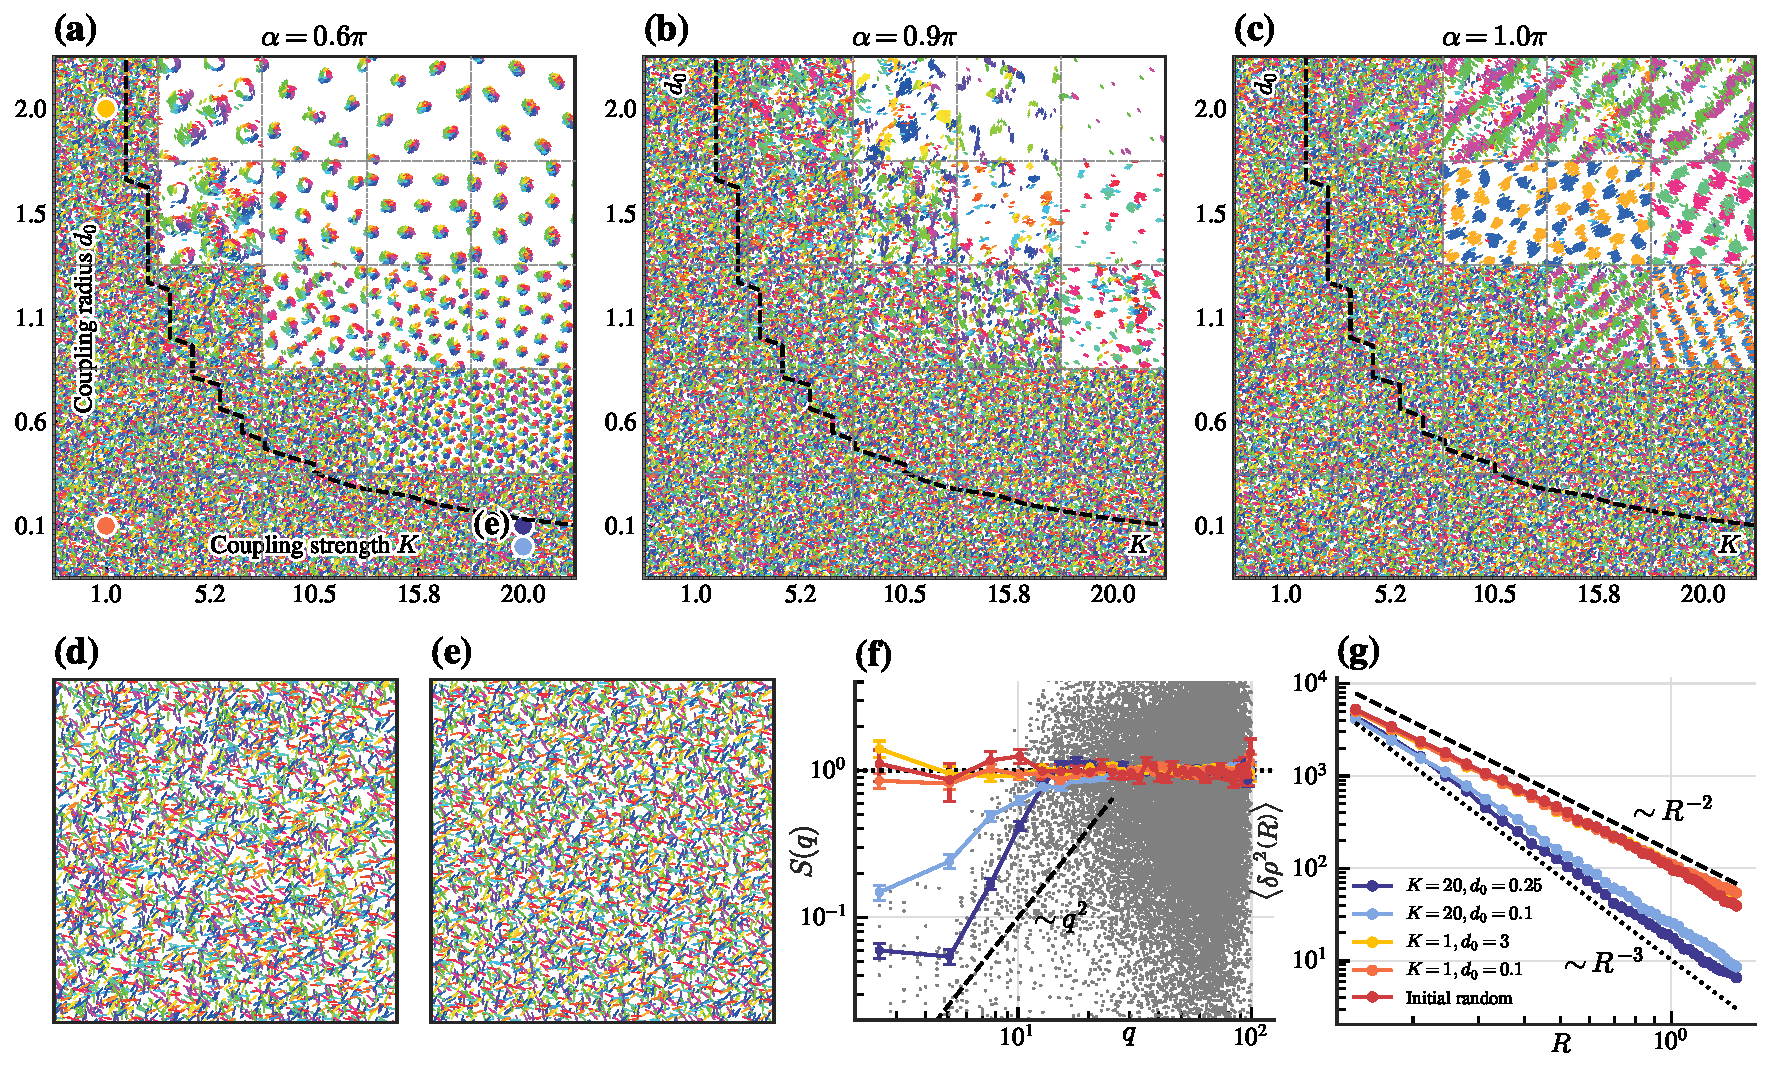
\includegraphics[width=\textwidth]{./figs/phaseDiagramAndHyperuniformity.pdf}
    \caption{
        \label{fig:phaseDiagramAndHyperuniformity}
        (a)-(c) Snapshots of $(K, d_0)$ phase diagram under different frustration $\alpha$ for $L=7, N=2000$ and $v=3$. The boundaries between dominant and recessive lattice states, are indicated with black dashed lines.
        (d), (e) Snapshots comparing random uniform initial conditions (d) and the resulting hyperuniform final state (e) for $K=20, d_0=0.25, \alpha=0.6\pi$ and $N=5000$ (large population for better showcase).
        Hyperuniformity of the recessive lattice states is characterized by the structure factor $S(q)$ in (f) and the density variance $\langle \delta \rho ^2\left( R \right) \rangle $ in (g). 
        Black dashed lines indicate the scaling behaviors $S(q)\sim q^{-2}$ and $\langle \delta \rho ^2\left( R \right) \rangle\sim R^{-2,-3}$, respectively.
        In (f), gray dots represent the sample of $S(\mathbf{q}_{\mathbf{n}})$ for periodic boundary conditions allowed wavevectors $\mathbf{q}_{\mathbf{n}}=(2\pi n_1/L,2\pi n_2/L)$ with $\mathbf{n}\in \left( \mathbb{Z} ^* \right) ^2$ at $K=20, d_0=0.25$, and the point-fold curves with error bars show the binned average and standard deviation of their respective $S(\mathbf{q}_{\mathbf{n}})$.
        Solid dots and text label in (a) mark the location in $(K, d_0)$ phase diagram corresponding to the parameters analyzed in (e)-(g).
    }
\end{figure}

\begin{figure}[H]
    \centering
    \includegraphics[width=\textwidth]{Figs/Sq_and_variance_rho.pdf}
    \caption{
        \label{fig:Sq_and_variance_rho}
        Structure factor scaling and density fluctuations across varying control parameters.
        (a) Structure factor $S(q)$ and (b) variance of density fluctuations $\langle \delta \rho ^2\left( R \right) \rangle$ for values of the frustration $\alpha / \pi$ at $K=24$. 
        The dashed lines indicate reference scaling behaviors for Poisson-like and hyperuniformity.
        Inset (c): The scaling exponent (slope) extracted from the curves in (b) plotted against $\alpha / \pi$.
        (d, e) Analogous plots to (a) and (b), respectively, showing the evolution of $S(q)$ and $\langle \delta \rho ^2\left( R \right) \rangle$ with increasing coupling strength $K$.
        Inset (f): The corresponding scaling exponent (slope) from (e) as a function of $K$.
        Other parameters: $d_0=0.25, v=3, L=7, N=5000$.
    }
\end{figure}   

\begin{figure}[H]
    \centering
    \includegraphics[width=\textwidth]{Figs/phase_bins_Sq_and_variance_rho.pdf}
    \caption{
        \label{fig:phase_bins_Sq_and_variance_rho}
        The impact of angular selectivity on global order and hyperuniformity. Particle configurations within specific angular ranges (a) exhibit distinct structural signatures, as quantified by the structure factor $S(q)$(b) and density fluctuations (c). 
        Parameters: $K=24, d_0=0.25, \alpha=0.8\pi, v=3, L=7, N=5000$.
    }
\end{figure} 

\begin{figure}[H]
    \centering
    \includegraphics[width=\textwidth]{Figs/slope_heatmap_and_hysteresis.pdf}
    \caption{
        \label{fig:slope_heatmap_and_hysteresis}
        Phase behavior and hysteresis of density fluctuation scaling. (a) Heat map of the scaling exponent of density fluctuations $\langle \delta \rho ^2\left( R \right) \rangle \sim R^{\lambda}$
        in the parameter space of coupling strength $K$ and frustration $\alpha/\pi$. The exponent $\lambda$ (color-coded) serves as an indicator of hyperuniformity ($\lambda \leqslant -2$) and other phases. (b, c) Hysteresis loops observed when sweeping the control parameter $K$ (b) and $\alpha/\pi$ (c), demonstrating second-order phase transitions between disordered and hyperuniform states.
        Other parameters are same as in Fig.~\ref{fig:Sq_and_variance_rho}.
    }
\end{figure} 


\bibliography{ref}

\end{document}